\subsection{Interrelación Departamento - Asesor Curso Académico}

   \begin{description}
      \item[Definición] En esta interrelación se deja constancia de que un
      asesor puede ofrecer servicios de asesoría perteneciendo a un departamento
      durante un determinado curso académico.

      \item[Características] La interrelación presenta las siguientes
                             características:

         \begin{itemize}
            \item \textbf{Nombre:} D-AseCA
            \item \textbf{Tipo de la interrelación:} El tipo de entidad
                  Asesor Curso Académico es débil por existencia respecto al
                  tipo de entidad Departamento.
            \item \textbf{Cardinalidad de la interrelación:} 1:N
                  \begin{itemize}
                     \item Departamento: dispone\_de (0,n)
                     \item Asesor Curso Académico: pertenece\_a (1,1)
                  \end{itemize}
            \item \textbf{Número de atributos:} Ninguno.
         \end{itemize}

      \item[Diagrama] La figura \ref{diagramaD-AseCA} muestra el diagrama de la
                      interrelación.

      \item \begin{figure}[!ht]
            \begin{center}
            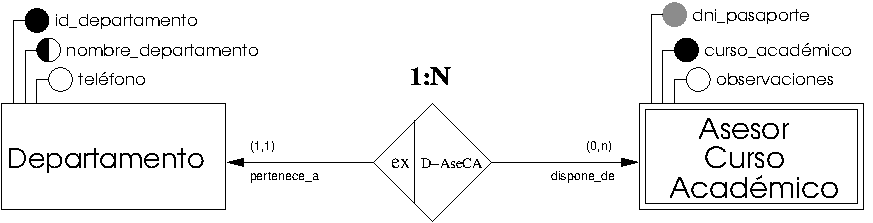
\includegraphics[]{07.Modelo_Entidad-Interrelacion/7.3.Analisis_Interrelaciones/diagramas/D-AseCA.pdf}
            \caption{Diagrama de la interrelación D-AseCA.}
            \label{diagramaD-AseCA}
            \end{center}
         \end{figure}

      \item[Ejemplo práctico del tipo de interrelación]

      \item \begin{center}
            \begin{tabular}{ | r r | }
            \hline
            \multicolumn{2}{ | c | }{\textbf{Tipo de interrelación D-AseCA}} \\
            \hline
            \textbf{Departamento} & \\
            id\_departamento & 22 \\
            \hline
            \textbf{Asesor Curso Académico} & \\
            dni\_pasaporte & 98765432Z \\
            curso\_académico & 2007 \\
            \hline
            \end{tabular}
         \end{center}
   \end{description}
